\section{Introduction}
\label{sec:intro}

Consider a bank that routes incoming customer messages to one of a fixed set of intents and sends a message to a
human whenever the routing model is less than 90\% confident. The threshold was chosen on validation data in which,
say, one message in ten was a complaint. After a service outage, four messages in ten are complaints. The model,
the messages of each kind and the threshold are unchanged; only the class frequencies have moved. Does the model's
confidence still mean what it meant at validation time, and does the threshold still send the intended share of
messages to a human?

This question has become practical for a new class of models. Typed decision models (TDMs), also called
``System One'' models, do not generate text: given an input and a caller-defined set of options, they return a
probability distribution over the options \citep{deusser2026jev,tang2026audit}. Jev is offered as a hosted API and
is described by its vendor as calibrated; Tev1-4B and Nimble-9B are open models fine-tuned from Qwen3.5 backbones
for the same interface. A trained classifier has a training prior that label-shift corrections can use
\citep{saerens2002adjusting,lipton2018detecting}. A zero-shot model has none. The closest substitute is an
\emph{implicit prior}: the average distribution the model predicts on a development set, which requires no labels.

Existing evaluations leave two gaps. First, the benefit of vendor ``decision training'' has not been separated from the
backbone: an audit of early TDM papers calls for same-backbone ablations \citep{tang2026audit}, existing comparisons of
a vendor TDM with its backbone read the two models out differently \citep{rafe2026systemone}, and the study that does
compare identical weights fine-tunes its own models and finds gains only on some tasks \citep{li2026llmasjev}. Second, TDMs have been compared with language models and trained classifiers at a
single class distribution \citep{deusser2026jev,rafe2026systemone}, so it is not known whether their calibration and
thresholds transfer when the class frequencies change; a recent audit of 28 TDM papers lists calibration under
deployment shift as an open problem \citep{tang2026audit}. Prior adaptation without labels has been studied for language
models and vision--language models \citep{estienne2023unsupervised,han2026labelshift}, but not for TDMs against trained
classifiers under controlled shift. We are not aware of a study that combines a commercial TDM, open TDMs paired with
their own backbones, trained classifiers and controlled prevalence shift with label-free prior correction
(\hyperref[tab:coverage]{Table~\ref*{tab:coverage}}); this combination is what allows us to ask what decision training adds and whether it
survives a change in class frequencies.

We study three research questions on five public, human-labelled datasets, using identical test items and
candidate sets for every system:
\textbf{RQ1} (decision training): does vendor decision training change accuracy and calibration relative to the same
backbone?
\textbf{RQ2} (prevalence shift): under controlled prevalence shift, do a TDM's calibration error and threshold risk
change differently from those of a fine-tuned classifier?
\textbf{RQ3} (implicit-prior correction): does expectation--maximisation (EM) prior correction with the implicit
prior reduce a TDM's calibration error under shift?
Our results concern \emph{candidate-set} decisions, in which the gold label is always among 3--22 offered options, and
\emph{simulated} label shift, in which only the class frequencies change; they do not cover full-label classification
over all 150 or 64 intents, or deployment shifts that also change the text of each class (\hyperref[sec:limitations]{Section~\ref*{sec:limitations}}).
The tests and the comparison family were fixed and hashed before the final runs, and the analysis before any test was
computed (\hyperref[sec:protocol]{Section~\ref*{sec:protocol}}); the one amendment, and earlier exposures of test data
during pipeline checks (mainly the FPB test split), are listed in \hyperref[app:deviations]{Appendix~\ref*{app:deviations}}.

Our findings are as follows (\hyperref[fig:teaser]{Figure~\ref*{fig:teaser}}; all 35 tests in \hyperref[tab:alltests]{Table~\ref*{tab:alltests}}).
\begin{itemize}
  \item \textbf{Decision training is task-dependent.} Nimble-9B, which differs from Qwen3.5-9B only by a LoRA
  adapter, is better calibrated on both intent datasets but 12.0 Macro-F1~points worse on financial sentiment, where
  its calibration error is also higher (\hyperref[sec:rq1]{Section~\ref*{sec:rq1}}). Tev1-4B is never significantly worse than
  Qwen3.5-4B, and is better on five of ten tests.
  \item \textbf{Moderate prevalence shift separates Jev from a fine-tuned classifier only a little.} At a Dirichlet
  concentration of $\alpha=1$, Jev's ECE and the excess risk of its confidence threshold grow significantly
  more than DeBERTa-v3-large's (after Holm correction) only on FPB, by 1.7 and 2.5 percentage points; averaged over
  2{,}000 shift scenarios (exploratory), the difference is at most one point on every dataset and largest on TREC-6 (\hyperref[sec:rq2]{Section~\ref*{sec:rq2}}).
  \item \textbf{Implicit-prior correction helps where calibration is poor.} EM with Jev's implicit prior, which needs
  no labels, lowers Jev's ECE under shift by 2.7~points on FPB and 1.8~points on HateXplain, the two datasets where its
  unshifted ECE is highest (0.095 and 0.279), with the same sign for every prior set; on the other three datasets the
  effect is not significant after Holm correction. Recalibration on labelled development data lowers the error much
  further (\hyperref[sec:rq3]{Section~\ref*{sec:rq3}}).
  \item \textbf{Artifacts.} We release the frozen label texts, candidate sets, prompts, evaluation code and every
  per-example probability vector \todo{repository link}.
\end{itemize}
In short, decision training helps a backbone on some tasks and hurts it on others, and prevalence shift matters less
for the TDMs we tested than the calibration error they already have without shift.

\begin{figure}[t]
  \centering
  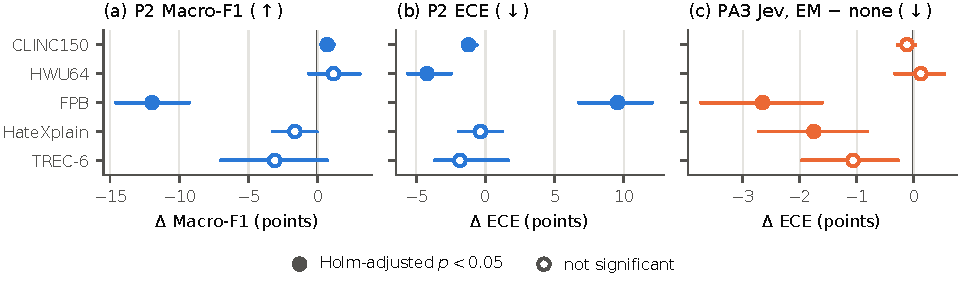
\includegraphics[width=\linewidth]{figures/fig1_teaser.pdf}
  \caption{\textbf{Decision training changes a backbone in a task-dependent direction, and label-free prior correction
  helps where calibration is poor.}
  (a, b) Paired differences between Nimble-9B and its own base model Qwen3.5-9B (same weights and 8-bit precision,
  differing only by a LoRA adapter) in Macro-F1 (higher favours Nimble) and expected calibration error (ECE; lower
  favours Nimble), in percentage points.
  (c) Change in Jev's ECE under prevalence shift ($\alpha=1$, 50 fixed target priors) when EM prior correction with
  its implicit prior is applied (lower is better).
  Bars are 95\% paired bootstrap intervals ($B=10{,}000$, unadjusted); filled markers are significant after Holm
  correction over all 35 primary tests.}
  \label{fig:teaser}
\end{figure}
